\setcounter{ProblemNumber}{1}
\textit{In problems 1--4, graph the solution set for each linear inequality.}\\
\ptwo{
\[3x+y < 4\]
\begin{center}
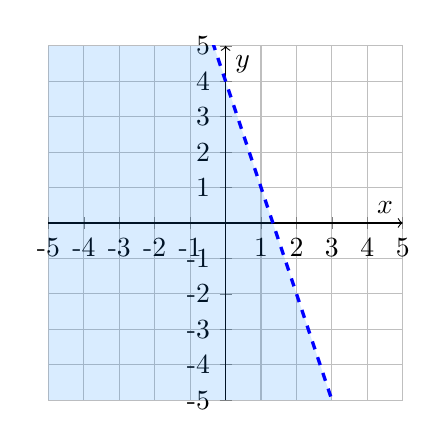
\begin{tikzpicture}
\begin{axis}[
    xmin=-5, xmax=5,
    ymin=-5, ymax=5,
    axis lines=center,
    axis on top=false,
    domain=0:1,
    x=0.45cm,
    y=0.45cm,
    xtick={-10,-9,...,10},
    xticklabels={-10,-9,...,10},
    ytick={-10,-9,...,10},
    yticklabels={-10,-9,...,10},
    axis lines=middle,
    axis line style={->},
    xlabel={$x$},
    ylabel={$y$},
    grid=major
    ]
    \addplot [thick,color=blue,fill=blue!50!cyan, 
                    fill opacity=0.15,draw opacity=0]coordinates {
            (-0.33,5)
            (-5,5)
            (-5,-5)
            (3,-5)  };
    \addplot [very thick,blue,dashed,domain=-10:10] {-3*x+4};	
\end{axis}
\end{tikzpicture}
\end{center}}
\ptwo{
\[x \geq y-2\]
\begin{center}
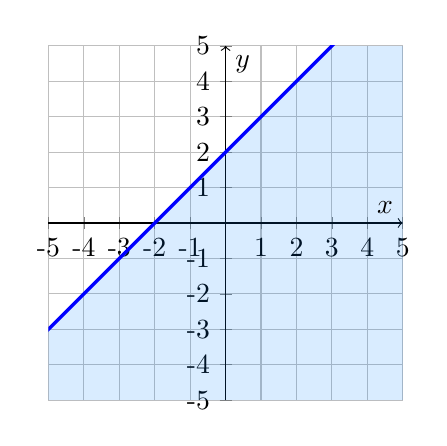
\begin{tikzpicture}
\begin{axis}[
    xmin=-5, xmax=5,
    ymin=-5, ymax=5,
    axis lines=center,
    axis on top=false,
    domain=0:1,
    x=0.45cm,
    y=0.45cm,
    xtick={-10,-9,...,10},
    xticklabels={-10,-9,...,10},
    ytick={-10,-9,...,10},
    yticklabels={-10,-9,...,10},
    axis lines=middle,
    axis line style={->},
    xlabel={$x$},
    ylabel={$y$},
    grid=major
    ]
    \addplot [thick,color=blue,fill=blue!50!cyan, 
                    fill opacity=0.15,draw opacity=0]coordinates {
            (-5,-3)
            (-5,-5)
            (5,-5)
            (5, 5)
            (3,5)  };
    \addplot [very thick,blue,domain=-10:10] {x+2};	
\end{axis}
\end{tikzpicture}
\end{center}}

\ptwo{
\[2x-2y > 4\]
\begin{center}
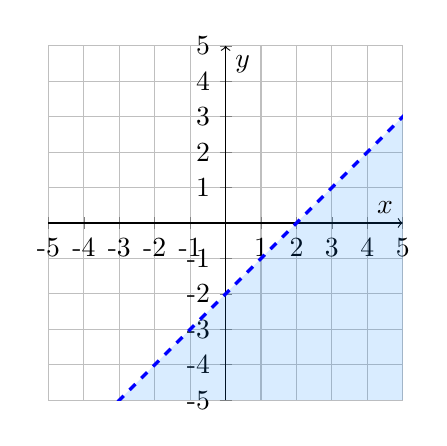
\begin{tikzpicture}
\begin{axis}[
    xmin=-5, xmax=5,
    ymin=-5, ymax=5,
    axis lines=center,
    axis on top=false,
    domain=0:1,
    x=0.45cm,
    y=0.45cm,
    xtick={-10,-9,...,10},
    xticklabels={-10,-9,...,10},
    ytick={-10,-9,...,10},
    yticklabels={-10,-9,...,10},
    axis lines=middle,
    axis line style={->},
    xlabel={$x$},
    ylabel={$y$},
    grid=major
    ]
    \addplot [thick,color=blue,fill=blue!50!cyan, 
                    fill opacity=0.15,draw opacity=0]coordinates {
            (5,3)
            (5,-5)
            (-3,-5)  };
    \addplot [very thick,blue,dashed,domain=-10:10] {x-2};	
\end{axis}
\end{tikzpicture}
\end{center}}
\ptwo{
\[y \leq \dfrac{1}{2}x-1\]
\begin{center}
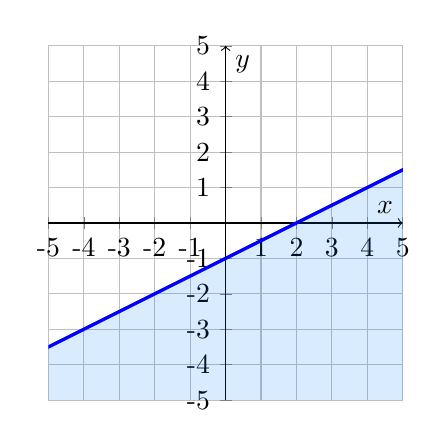
\begin{tikzpicture}
\begin{axis}[
    xmin=-5, xmax=5,
    ymin=-5, ymax=5,
    axis lines=center,
    axis on top=false,
    domain=0:1,
    x=0.45cm,
    y=0.45cm,
    xtick={-10,-9,...,10},
    xticklabels={-10,-9,...,10},
    ytick={-10,-9,...,10},
    yticklabels={-10,-9,...,10},
    axis lines=middle,
    axis line style={->},
    xlabel={$x$},
    ylabel={$y$},
    grid=major
    ]
    \addplot [thick,color=blue,fill=blue!50!cyan, 
                    fill opacity=0.15,draw opacity=0]coordinates {
            (5,1.5)
            (5,-5)
            (-5,-5)
            (-5,-3.5)  };
    \addplot [very thick,blue,domain=-10:10] {x/2-1};	
\end{axis}
\end{tikzpicture}
\end{center}}

\textit{In problems 5--12, graph the solution set for each system of inequalities.}\\
\ptwo{
\begin{align*}
x-3y &> -6\\
x &\leq -3
\end{align*}
\begin{center}
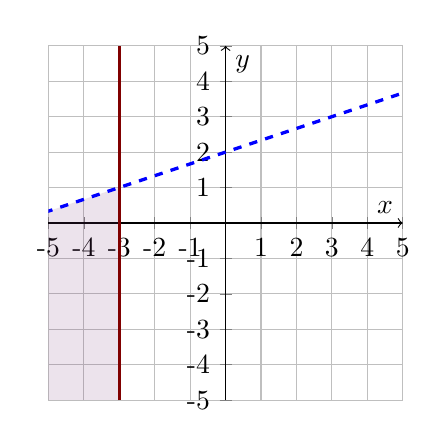
\begin{tikzpicture}
\begin{axis}[
    xmin=-5, xmax=5,
    ymin=-5, ymax=5,
    axis lines=center,
    axis on top=false,
    domain=0:1,
    x=0.45cm,
    y=0.45cm,
    xtick={-10,-9,...,10},
    xticklabels={-10,-9,...,10},
    ytick={-10,-9,...,10},
    yticklabels={-10,-9,...,10},
    axis lines=middle,
    axis line style={->},
    xlabel={$x$},
    ylabel={$y$},
    grid=major
    ]
    \addplot [thick,color=blue,fill=blue!50!cyan!50!red, 
                    fill opacity=0.15,draw opacity=0]coordinates {
            (-3,1)
            (-3,-5)
            (-5,-5)
            (-5,1/3)  };
	\addplot [very thick,blue,dashed,domain=-10:10] {x/3+2};
	\addplot [very thick,red!50!black] coordinates{(-3,-5)(-3,5)};
\end{axis}
\end{tikzpicture}
\end{center}}
\ptwo{
\begin{align*}
3x+4y &< 12\\
y &\geq -2x+1
\end{align*}
\begin{center}
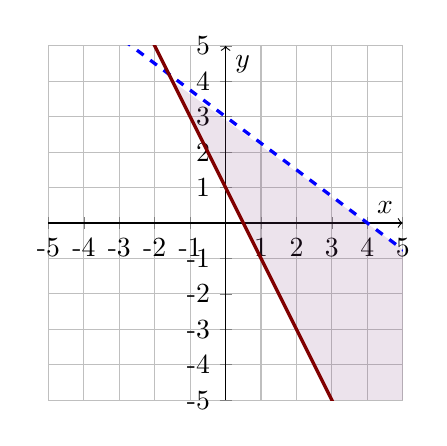
\begin{tikzpicture}
\begin{axis}[
    xmin=-5, xmax=5,
    ymin=-5, ymax=5,
    axis lines=center,
    axis on top=false,
    domain=0:1,
    x=0.45cm,
    y=0.45cm,
    xtick={-10,-9,...,10},
    xticklabels={-10,-9,...,10},
    ytick={-10,-9,...,10},
    yticklabels={-10,-9,...,10},
    axis lines=middle,
    axis line style={->},
    xlabel={$x$},
    ylabel={$y$},
    grid=major
    ]
    \addplot [thick,color=blue,fill=blue!50!cyan!50!red, 
                    fill opacity=0.15,draw opacity=0]coordinates {
            (5, -3/4)
            (-1.5,4)
            (3,-5)
            (5,-5)  };
	\addplot [very thick,blue,dashed,domain=-10:10] {-3*x/4+3};
	\addplot [very thick,red!50!black,domain=-10:10] {-2*x+1};
\end{axis}
\end{tikzpicture}
\end{center}}

\ptwo{
\begin{align*}
x &\geq y-3\\
y &> 2x+1
\end{align*}
\begin{center}
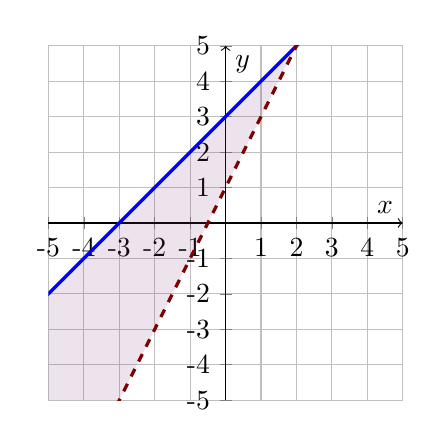
\begin{tikzpicture}
\begin{axis}[
    xmin=-5, xmax=5,
    ymin=-5, ymax=5,
    axis lines=center,
    axis on top=false,
    domain=0:1,
    x=0.45cm,
    y=0.45cm,
    xtick={-10,-9,...,10},
    xticklabels={-10,-9,...,10},
    ytick={-10,-9,...,10},
    yticklabels={-10,-9,...,10},
    axis lines=middle,
    axis line style={->},
    xlabel={$x$},
    ylabel={$y$},
    grid=major
    ]
    \addplot [thick,color=blue,fill=blue!50!cyan!50!red, 
                    fill opacity=0.15,draw opacity=0]coordinates {
            (-5, -2)
            (2,5)
            (-3,-5)
            (-5,-5)  };
	\addplot [very thick,blue,domain=-10:10] {x+3};
	\addplot [very thick,red!50!black,dashed,domain=-10:10] {2*x+1};
\end{axis}
\end{tikzpicture}
\end{center}}
\ptwo{
\begin{align*}
y &> -4\\
x &\leq 2
\end{align*}
\begin{center}
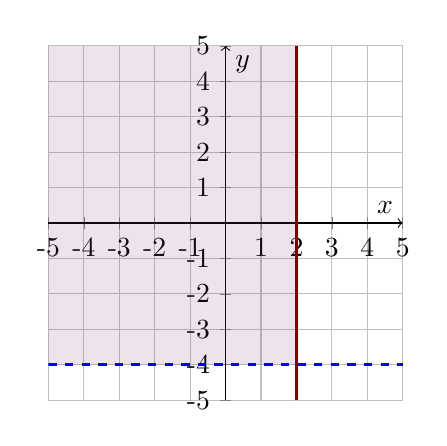
\begin{tikzpicture}
\begin{axis}[
    xmin=-5, xmax=5,
    ymin=-5, ymax=5,
    axis lines=center,
    axis on top=false,
    domain=0:1,
    x=0.45cm,
    y=0.45cm,
    xtick={-10,-9,...,10},
    xticklabels={-10,-9,...,10},
    ytick={-10,-9,...,10},
    yticklabels={-10,-9,...,10},
    axis lines=middle,
    axis line style={->},
    xlabel={$x$},
    ylabel={$y$},
    grid=major
    ]
    \addplot [thick,color=blue,fill=blue!50!cyan!50!red, 
                    fill opacity=0.15,draw opacity=0]coordinates {
            (2,5)
            (-5,5)
            (-5,-4)
            (2,-4)  };
	\addplot [very thick,blue,dashed] coordinates{(-5,-4)(5,-4)};
	\addplot [very thick,red!50!black] coordinates{(2,-5)(2,5)};
\end{axis}
\end{tikzpicture}
\end{center}}

\ptwo{
\begin{align*}
x+y &> -4\\
x-y &\leq 0
\end{align*}
\begin{center}
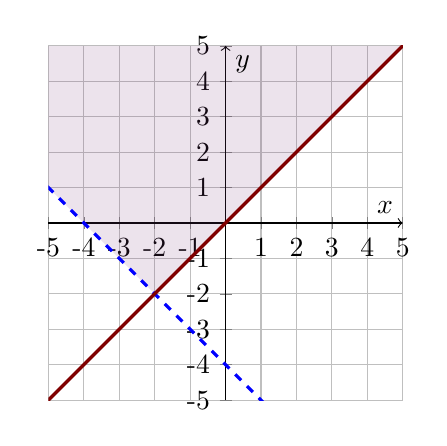
\begin{tikzpicture}
\begin{axis}[
    xmin=-5, xmax=5,
    ymin=-5, ymax=5,
    axis lines=center,
    axis on top=false,
    domain=0:1,
    x=0.45cm,
    y=0.45cm,
    xtick={-10,-9,...,10},
    xticklabels={-10,-9,...,10},
    ytick={-10,-9,...,10},
    yticklabels={-10,-9,...,10},
    axis lines=middle,
    axis line style={->},
    xlabel={$x$},
    ylabel={$y$},
    grid=major
    ]
    \addplot [thick,color=blue,fill=blue!50!cyan!50!red, 
                    fill opacity=0.15,draw opacity=0]coordinates {
            (-5, 1)
            (-5,5)
            (5,5)
            (-2,-2)  };
	\addplot [very thick,blue,dashed,domain=-10:10] {-x-4};
	\addplot [very thick,red!50!black,domain=-10:10] {x};
\end{axis}
\end{tikzpicture}
\end{center}}
\ptwo{
\begin{align*}
2x-5y &\leq -10\\
y &< 3
\end{align*}
\begin{center}
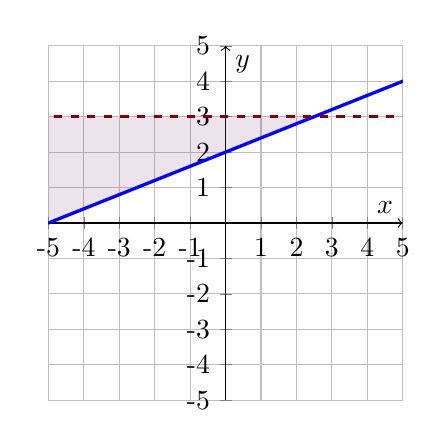
\begin{tikzpicture}
\begin{axis}[
    xmin=-5, xmax=5,
    ymin=-5, ymax=5,
    axis lines=center,
    axis on top=false,
    domain=0:1,
    x=0.45cm,
    y=0.45cm,
    xtick={-10,-9,...,10},
    xticklabels={-10,-9,...,10},
    ytick={-10,-9,...,10},
    yticklabels={-10,-9,...,10},
    axis lines=middle,
    axis line style={->},
    xlabel={$x$},
    ylabel={$y$},
    grid=major
    ]
    \addplot [thick,color=blue,fill=blue!50!cyan!50!red, 
                    fill opacity=0.15,draw opacity=0]coordinates {
            (-5, 3)
            (2.5,3)
            (-5,0)  };
	\addplot [very thick,blue,domain=-10:10] {2*x/5+2};
	\addplot [very thick,red!50!black,dashed,domain=-10:10] {3};
\end{axis}
\end{tikzpicture}
\end{center}}

\ptwo{
\begin{align*}
4x+5y &< 20\\
y &> -\dfrac{1}{3}x+2
\end{align*}
\begin{center}
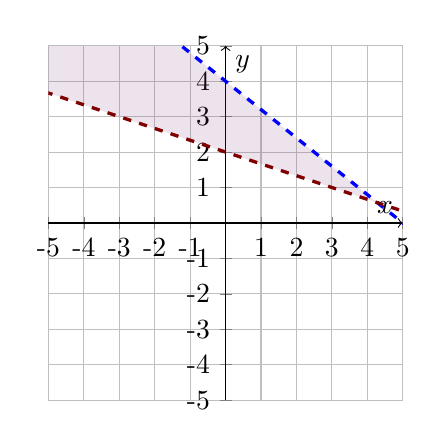
\begin{tikzpicture}
\begin{axis}[
    xmin=-5, xmax=5,
    ymin=-5, ymax=5,
    axis lines=center,
    axis on top=false,
    domain=0:1,
    x=0.45cm,
    y=0.45cm,
    xtick={-10,-9,...,10},
    xticklabels={-10,-9,...,10},
    ytick={-10,-9,...,10},
    yticklabels={-10,-9,...,10},
    axis lines=middle,
    axis line style={->},
    xlabel={$x$},
    ylabel={$y$},
    grid=major
    ]
    \addplot [thick,color=blue,fill=blue!50!cyan!50!red, 
                    fill opacity=0.15,draw opacity=0]coordinates {
            (-5, 11/3)
            (-5,5)
            (-5/4,5)
            (30/7,4/7)  };
	\addplot [very thick,blue,dashed,domain=-10:10] {-4*x/5+4};
	\addplot [very thick,red!50!black,dashed,domain=-10:10] {-x/3+2};
\end{axis}
\end{tikzpicture}
\end{center}}
\ptwo{
\begin{align*}
y &> \dfrac{3}{5}x-4\\
y &\leq -\dfrac{4}{3}x+3
\end{align*}
\begin{center}
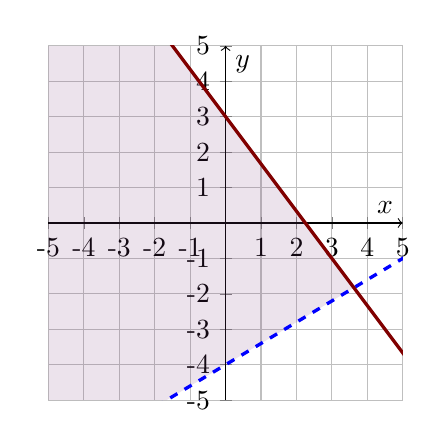
\begin{tikzpicture}
\begin{axis}[
    xmin=-5, xmax=5,
    ymin=-5, ymax=5,
    axis lines=center,
    axis on top=false,
    domain=0:1,
    x=0.45cm,
    y=0.45cm,
    xtick={-10,-9,...,10},
    xticklabels={-10,-9,...,10},
    ytick={-10,-9,...,10},
    yticklabels={-10,-9,...,10},
    axis lines=middle,
    axis line style={->},
    xlabel={$x$},
    ylabel={$y$},
    grid=major
    ]
    \addplot [thick,color=blue,fill=blue!50!cyan!50!red, 
                    fill opacity=0.15,draw opacity=0]coordinates {
            (-5, 5)
            (-1.5,5)
            (105/29,-53/29)
            (-5/3,-5)
            (-5,-5)  };
	\addplot [very thick,blue,dashed,domain=-10:10] {3*x/5-4};
	\addplot [very thick,red!50!black,domain=-10:10] {-4*x/3+3};
\end{axis}
\end{tikzpicture}
\end{center}}